\documentclass[12pt,letterpaper]{standalone}
\usepackage{pgf, tikz}
\usetikzlibrary{arrows, automata}
\usepackage{mwe} % For dummy images 
\usetikzlibrary{positioning}
\usepackage{tikz-uml}

\begin{document}
	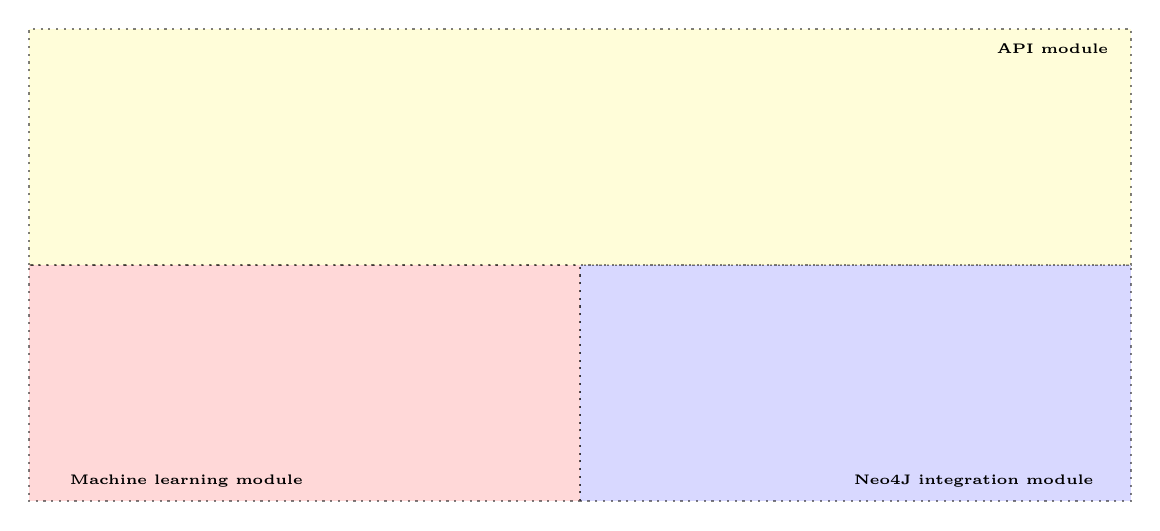
\begin{tikzpicture}
	
		\draw[fill=blue!30, dotted, thick, semitransparent] (0,0) rectangle (7, 3); 
		\draw[fill=red!30, dotted, thick, semitransparent] (0,0) rectangle (-7, 3); 
		\draw[fill=yellow!30, dotted, thick, semitransparent] (-7,3) rectangle (7, 6); 
		
		\node at (5,.25) {\bf \tiny{Neo4J integration module}};
		\node at (-5,.25) {\bf \tiny{Machine learning module}};
		\node at (6,5.75) {\bf \tiny{API module}}; 
		
		\umlclass[x=0, y=4.7, alias=RequestJob, fill=blue!10, type=abstract]{server.jobs.RequestJob} {
			...
		} {
			...
		}
	
		\umlclass[x=-3.5, y=1.6, alias=Model, fill=yellow!10, type=abstract]{models.Model} {
			...
		} {
			...
		}
	
		\umlclass[x=3.5, y=1.6, alias=DatabaseDriver, fill=orange!10, type=abstract]{data.neo4j.DatabaseDriver} {
			...
		} {
			...
		}
	
		\umlassoc[thick]{RequestJob}{Model} 
		\umlassoc[thick]{RequestJob}{DatabaseDriver} 
	\end{tikzpicture}
\end{document}